% =========================================================
% 1. Introduction to ORM Methods
% =========================================================
\section{Introduction to ORM Methods}

\begin{frame}[standout]
  Introduction to ORM\\Methods
\end{frame}

\begin{frame}[fragile]{WHAT IS ORM?}
  \begin{itemize}
    \item The ORM stands for \textbf{Object Relational Mapping}.
    \item It is a programming technique that allows developers to interact with a
          database using Python objects and methods instead of writing SQL queries
          \textbf{directly}.
    \item In Odoo, the ORM acts as a bridge between the Python application and the
          PostgreSQL database.
    \item Instead of writing:
  \end{itemize}
\begin{lstlisting}[language=SQL]
INSERT INTO student_student (name, age) VALUES ('Ahmed', 22);
\end{lstlisting}
  \begin{itemize}
    \item we simply write:
  \end{itemize}
\begin{lstlisting}
self.env['student.student'].create({
    'name': 'Ahmed',
    'age': 22,
})
\end{lstlisting}
\end{frame}

\begin{frame}[fragile]{WHAT DOES ``OBJECT RELATIONAL MAPPING'' MEAN?}
  \begin{itemize}
    \item The term consists of three parts.
  \end{itemize}
  \begin{enumerate}
    \item \textbf{Object} -- an object is an instance of a Python class.
\begin{lstlisting}
student = self.env['student.student'].browse(1)
\end{lstlisting}
          Here, \texttt{student} is a Python object representing a student.
    \item \textbf{Relational} -- a relational database stores data in tables that are
          connected using relationships.\\[0.2em]
          Students $\leftrightarrow$ Classes \quad (e.g.\ Mohamed $\leftrightarrow$ Grade 12)
    \item \textbf{Mapping} -- mapping means connecting two different worlds.\\[0.2em]
          Python Object $\Rightarrow$ Odoo ORM $\Rightarrow$ PostgreSQL Table
  \end{enumerate}
\end{frame}

\begin{frame}{ORM ARCHITECTURE}
  \begin{center}
    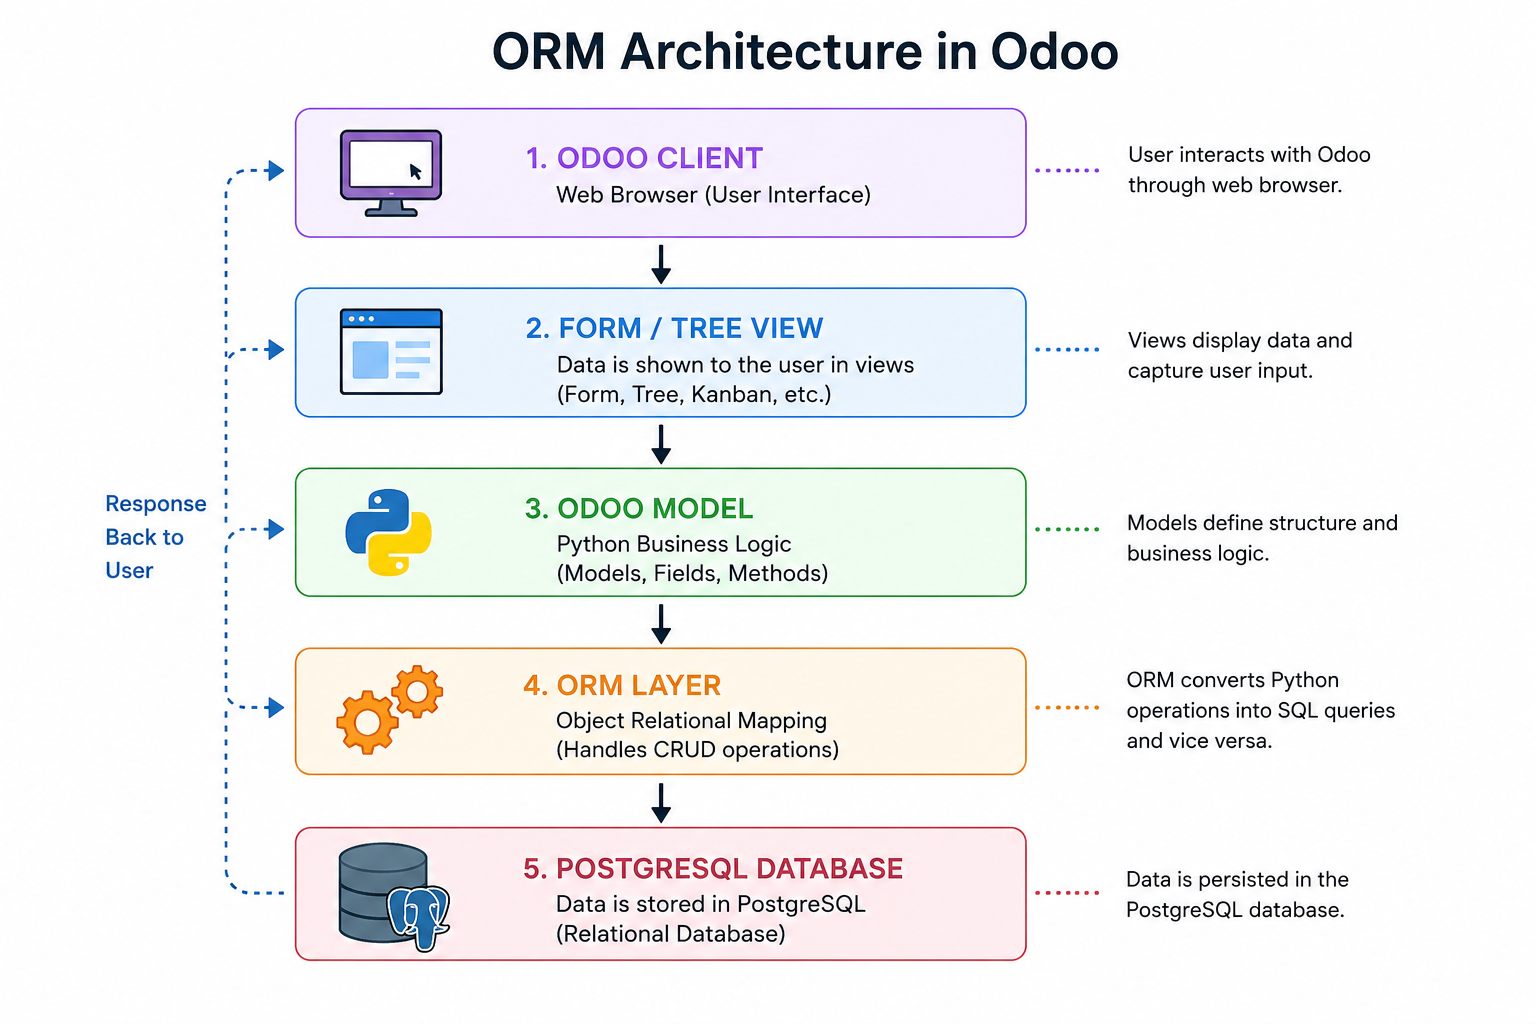
\includegraphics[width=0.92\textwidth,height=0.78\textheight,keepaspectratio]{assets/orm_architecture.png}
  \end{center}
\end{frame}

\begin{frame}{WHY IS ORM IMPORTANT?}
  \begin{itemize}
    \item Without an ORM, developers would need to:
      \begin{itemize}
        \item Write SQL for every operation.
        \item Manage database connections manually.
        \item Convert database rows into Python objects.
        \item Prevent SQL injection.
      \end{itemize}
    \item Although powerful, the ORM has limitations.
      \begin{itemize}
        \item Less control over complex SQL queries.
        \item Very large reports may require raw SQL.
        \item Advanced database tuning sometimes needs direct SQL.
      \end{itemize}
  \end{itemize}
\end{frame}

\begin{frame}{COMMON ORM METHODS}
  \begin{columns}[T]
    \begin{column}{0.48\textwidth}
      \begin{itemize}
        \item \texttt{create}
        \item \texttt{write}
        \item \texttt{unlink}
        \item \texttt{copy}
        \item \texttt{exists}
        \item \texttt{search}
        \item \texttt{read}
        \item \texttt{search\_read}
        \item \texttt{search\_count}
        \item \texttt{name\_create}
      \end{itemize}
    \end{column}
    \begin{column}{0.48\textwidth}
      \begin{itemize}
        \item \texttt{default\_get}
        \item \texttt{name\_search}
        \item \texttt{get\_view()}
        \item \texttt{ensure\_one()}
        \item \texttt{filtered()}
        \item \texttt{mapped()}
        \item \texttt{sorted()}
        \item \texttt{grouped()}
        \item \texttt{fields\_get()}
        \item \texttt{get\_metadata}
      \end{itemize}
    \end{column}
  \end{columns}
\end{frame}
